\chapter{Implementácia}  % chapter* je necislovana kapitola
\label{implementacia}

Implementácia je realizovaná v programovacom jazyku \textit{Python 3} s využitím dodatočných knižníc na podporu tvorby modelov strojového učenia, spracovania a analýzy dátových sád a iné:
\begin{itemize}
    \item \textbf{sys} - knižnica podpory prístupu k systemovým zdrojom
    \item \textbf{os} -  knižnica podpory prístupu k operačnému systému
    \item \textbf{Keras} - knižnica podpory tvorby modelov strojového učenia
    \item \textbf{Tensorflow} - knižnica podpory tvorby modelov strojového učenia a prístupu k algoritmom trénovania modelov strojového učenia
    \item \textbf{Pandas} - knižnica podpory spracovania a analýzy dátových sád
    \item \textbf{Numpy} - knižnica podpory zložitých matematických operácií nad dátovými sadami
    \item \textbf{scikit learn} - knižnica podpory tvorby modelov strojového učenia a operácií nad dátovými sadami
    \item \textbf{random} - knižnica podpory generovania náhodných čísel
\end{itemize}

Zdrojový kód programu je implementovaný vo forme python skriptu. Výstupom skriptu sú dátové súbory, ktoré obsahujú:
\begin{enumerate}
    \item zdrojové vzorky kalibrované pomocou MMD-ResNet využívajúcej algoritmus syntetického gradientu (vo formáte \mintinline{Python}{csv})
    \item predikované triedy jednotlivých buniek zdrojových vzoriek (vo formáte \mintinline{Python}{csv})
    \item vizualizácia priebehu vývoja hodnoty MMD v čase trénovania MMD-ResNet (vo formáte \mintinline{Python}{png})
    \item vizualizácia priebehu vývoja hodnoty MMD v jednotlivých iteráciách trénovania MMD-ResNet (vo formáte \mintinline{Python}{png})
    \item vizualizácia vývoja \textit{F1 skóre} v priebehu trénovania MMD-ResNet (vo formáte \mintinline{Python}{png})
\end{enumerate}

Kód programu bol vyvíjaný vo vývojovom prostredí \textit{Spyder IDE} určenom na tvorbu python skriptov. Testovanie implementácie bolo realizované prostredníctvom webovej služby \textit{Google Colaboratory} (dostupnej na adrese \url{https://colab.research.google.com/}). Webovú službu \textit{Google Colaboratory} sme využili z dôvodu bezplatného prístupu k supervýkonným grafickým akcelerátorom \textit{NVIDIA\textsuperscript{\textregistered} Tesla}, ktoré umožnili rýchlejšie a efektívnejšie vykonávanie zložitých matematických operácií (viac v Kap. \ref{vysledky}). 

\section{Implementácia metódy DeepCyTOF}
\label{impl_deepcytof}

Pri našej implementácii metódy DeepCyTOF sme vychádzali z pôvodnej implementácie, ktorú zverejnil zdroj \cite{Li2017} na adrese \url{https://github.com/KlugerLab/deepcytof}. Vzhľadom na úspešnosť tejto metódy pri automatickom gatovaní \cite{Li2016, Li2017}, sme sa rozhodli čo najmenej upravovať pôvodnú konfiguráciu jednotlivých komponentov metódy DeepCyTOF. Naším cieľom je nehradenie pôvodnej reziduálnej siete MMD-ResNet za nami vytvorenú reziduálnu sieť MMD-ResNet, ktorá pri trénovaní využíva algoritmus syntetického gradientu.

Pôvodná implementácia, ktorú zverejnil \cite{Li2017} obsahuje hlavný skript (súbor) \textit{DeepCyTOF.py} a niekoľko ďalších súborov, ktoré obsahujú nevyhnutné funkcionálne prvky použité pri realizácii automatického gatovania. Pri spustení hlavného skriptu je načítaná všetká potrebná konfigurácia:
\begin{enumerate}
    \item isCalibrate - zadefinovanie, či je potrebné kalibrovať vstupné dáta. Predvoilená hodnota \textit{true}.
    \item denoise - zadefinovanie, či je potrebné nahradiť chýbajúce hodnoty vo vstupných dátach. Predvolená hodnota \textit{true}.
    \item loadModel - zadefinovanie, či je potrebné načítať existujúci model z disku alebo natrénovať nový model. Platí pre všetky neurónové siete obsiahnuté v metóde DeepCyTOF. Predvolená hodnota \textit{false}.
    \item hiddenLayersSizes - pole veľkostí skrytých vrstiev klasifikátora (doprednej neurónovej siete). Predvolené hodnoty 12, 6 a 3.
    \item activation - aktivačná funkcia na skrytých vrstiev bunkového klasifikátora. Predovlená hodnota softplus \cite{Goh1995}.
    \item l2\_penalty - hodnota \textit{$L_2$} regularizácie váh skrytých vrstiev \cite{Goh1995}. Platí pre všetky neurónové siete obsiahnuté v metóde DeepCyTOF. Predvolená hodnota $10^{-4}$.
\end{enumerate}

Po inicializácii konfigurácie je pomocou funkcie \mintinline{Python}{Session()} vytvorené virtuálne pamäťové prostredie v ktorom sa vykonávajú operácie a výpočty nad modelmi strojového učenia. Dané virtuálne pamäťové prostredie obsahuje hodnoty všetkých váh, všetkých neurónových sieti, ktoré sú v tomto prostredí inicializované. Funkcia \mintinline{Python}{Session()} je súčasťou knižnice \textit{TensorFlow} (ďalej len tf). Po inicializácii virtuálneho pamäťového prostredia je dané prostredie použité ako predvolené virtuálne pamäťové prostredie, pomocou funkcie \mintinline{Python}{K.set_session()}, ktorá berie ako parameter inicializované virtuálne pamäťové prostredie. Funkcia \mintinline{Python}{K.set_session()} je súčasťou knižnice \textit{Keras} (ďalej len K)

Po vytvorení virtuálneho pamäťového prostredia je spomedzi všetkých vzoriek v dátovej sade vybraná jedna referenčná vzorka. Výber referenčnej vzorky je realizovaný funkciou \mintinline{Python}{chooseReferenceSample}, obsiahnutou v súbore \mintinline{Python}{DataHandler.py}. Daná metóda berie ako parameter cestu k jednotlivým vzorkám, čísla vzoriek, ktoré budú použité pri trénovaní neurónových sieti, identifikátory markerov, ktoré sú relevantné pre vybraný dataset, formát súborov vzoriek, počet riadkov, ktorý má byť ignorovaný pri načítaní vzorky (v prípade ak vzorka obsahuje názvy jednotlivých atribútov) a identifikátor, ktorý definuje, či je pre danú vzorku dostupná supervízia. Realizácia výberu referenčnej vzorky je opísaná v Kap. \ref{feed-forward-classifikator}.

Vybraná referenčná vzorka je následne načítaná do pamäte pomocou funkcie \mintinline{Python}{loadDeepCyTOFData}, obsiahnutej v súbore \mintinline{Python}{DataHandler.py}. Referenčná vzorka sa načíta do pamäte ako inštancia triedy \mintinline{Python}{Sample}, ktorá má atribúty:
\begin{itemize}
    \item \mintinline{Python}{X} - hodnoty markerov pre danú vzorku
    \item \mintinline{Python}{y} - identifikátor skupiny buniek pre danú vzorku (supervízia)
\end{itemize}
Po načítaní referenčnej vzorky do pamäte je vykonaná logaritmická transformácia hodnôt markerov ako:
\begin{equation}
\label{log_transf}
    A_{i,j} = log(1+|A_{i,j}|),
\end{equation}
Logaritmická transformácia hodnôt markerov je realizovaná funkciou \mintinline{Python}{preProcessSamplesCyTOFData()}, obsiahnutou v súbore \mintinline{Python}{DataHandler.py}, ktorá ako parameter prijíma objekt triedy \mintinline{Python}{Sample}. 

Referenčná vzorka je po absolvovaní logaritmickej transformácie použitá na trénovanie odšumujúceho autoenkódera (DAE). Trénovanie DAE je realizované funkciou \mintinline{Python}{trainDAE()}, obsiahnutou v súbore \mintinline{Python}{denoisingAutoEncoder.py}. Funkcia \mintinline{Python}{trainDAE()} prijíma ako parameter referenčnú vzorku, ktorá je použitá na trénovanie autoenkódera, cestu k jednotlivým vzorkám dátovej sady, identifikátor referenčnej vzorky, identifikátory vzoriek obsiahnutých v dátovej sade, zoznam relevantných markerov, formát súboru, v ktorom sú uložené vzorky dátovej sady, hodnota pravdepodobnosti ponechania jednotlivých buniek z vybranej vzorky, ktorá bude použitá pri trénovaní DAE, identifikátor, ktorý definuje, či je potrebné nahradiť chýbajúce hodnoty v dátovej sade, identifikátor, ktorý definuje, či je potrebné trénovať nový DAE alebo je možné načítať ho z disku a cesta, kde sa má DAE po natrénovaní uložiť. Podrobnejšie vysvetlenie implementácie trénovania DAE je uvedené v Prílohe \ref{train_DAE}. 

Po natrénovaní DAE nastáva fáza odšumenia referenčnej vzorky, pri ktorej sú nahradené chýbajúce hodnoty za reálne čísla. Odšumenie referenčnej vzorky je realizované funkciou \mintinline{Python}{predictDAE()}, obsiahnutou v súbore \mintinline{Python}{denoisingAutoEncoder.py}.  Funkcia \mintinline{Python}{predictDAE()} prijíma ako parametre natrénovaný DAE (resp. objekt triedy \mintinline{Python}{Model} obsiahnutý v knižnici \mintinline{Python}{Keras}), identifikátor, ktorý definuje, či je potrebné odšumovať vstupné dáta a vstupné dáta - objekt triedy \mintinline{Python}{Sample}, ktorého hodnoty atribútu \mintinline{Python}{X} sú odšumené. Podrobnejšie vysvetlenie implementácie odšumenia vstupných dát pomocou DAE je uvedené v Prílohe \ref{predict_DAE}. 
 
Odšumené dáta sú následne štandardizované pomocou funkcie \mintinline{Python}{standard_scale()}, obsiahnutej v súbore \mintinline{Python}{DataHandler.py}. Štandardizácia dát škáluje dáta tak, aby priemer hodnôt jednotlivých parametrov bol rovný nule:
\[
z = \frac{x-\bar{x}}{\sigma}
\]
kde $x$ sú vstupné dáta, $\bar{x}$ je priemer hodnôt vstupných dát a $\sigma$ je štandardná odchylka. Funkcia \mintinline{Python}{standard_scale()} prijíma ako parametre vstupné dáta ktoré sú štandardizované a model (objekt inštancie \mintinline{Python}{preprocessing}, obsiahnutý v knižnici Scikit Learn), ktorý je použitý na štandardizovanie vstupných dát (voliteľné). Ak model nie je dostupný, tak je inicializovaný a trénovaný nový model. Výstupom funkcie \mintinline{Python}{standard_scale()} sú štandardizované dáta a model, ktorým boli vstupné dáta štandardizované.

Štandardizované dáta sú následne použité na trénovanie bunkového klasifikátora (jednoduchej doprednej neurónovej siete). Ak nie je potrebné trénovať nový model bunkového klasifikátora, tak je klasifikátor načítaný z disku. Bunkový klasifikátor je trénovaný pomocou volania funkcie \mintinline{Python}{trainClassifier()}, obsiahnutej v súbore \mintinline{Python}{feedforwardClassifier.py}. Funkcia \mintinline{Python}{trainClassifier()} prijíma ako parametre odšumené dáta, ktoré sú použité na trénovanie klasifikátora, pole veľkostí skrytých vrstiev klasifikátora, aktivačnú funkciu na výstupe klasifikátora, hodnotu $L_2$ regularizácie váh skrytých vrstiev a cestu, kde bude novo-natrénovaný klasifikátor uložený. Podrobnejšie vysvetlenie implementácie trénovania bunkového klasifikátora je uvedené v Prílohe \ref{trainFF}.

Po natrénovaná bunkového klasifikátora je možné prejsť k automatického gatovaniu všetkých vzoriek z dátovej sady. Iterovaním po jednotlivých vzorkách z dátovej sady sú dané vzorky načítané do pamäte (funkciou \mintinline{Python}{loadDeepCyTOFData()}), normalizované pomocou logaritmickej transformácie (funkciou \mintinline{Python}{preProcessSamplesCyTOFData()}), odšumené pomocou natrénovaného DAE (funkciou \mintinline{Python}{predictDAE()}) a štandardizované pomocou modelu netrénovanom na referenčnej vzorke (funkciou \mintinline{Python}{standard_scale()}). Iterovaním po jednotlivých vzorkách dátovej sady sú vykonané rovnaké transformácie ako pri predspracovani referenčnej vzorky. 

Po dokončení predspracovania zdrojových vzoriek (jednotlivých vzoriek dátovej sady okrem referenčnej vzorky), je vykonané gatovanie na danej vzorke pomocou natrénovaného bunkovanie klasifikátora. Gatovanie zdrojovej vzorku je realizované funkciou \mintinline{Python}{prediction()}, obsiahnutej v súbore \mintinline{Python}{feedforwardClassifier.py}. Funkcia \mintinline{Python}{prediction()} prijíma ako parametre dáta ktoré budú gatované (hodnoty markerov) a natrénovaný klasifikátor, ktorý bude použitý na gatovanie (resp. objekt triedy \mintinline{Python}{Model}, obsiahnutej v knižnici \mintinline{Python}{Keras}). Podrobnejšie vysvetlenie implementácie predikcie vstupných dát pomocou bunkového klasifikátora je uvedené v Prílohe \ref{gateFF}.

Na kalibráciu hodnôt markerov je inicializovaná inštancia triedy \mintinline{Python}{ModelSG}, obsiahnutej v súbore \mintinline{Python}{MMDNet_SG.py}. Inštancia triedy \mintinline{Python}{ModelSG} je inštanciou reziduálnej siete s chybovou funkciou \mintinline{Python}{MMD()}, ktorá je trénovaná algoritmom syntetického gradientu. Inicializácia objektu triedy \mintinline{Python}{ModelSG} vyžaduje nasledujúce informácie:
\begin{enumerate}
    \item Odšumená referenčná vzorka - využitá pri vyrátavaní hodnoty MMD medzi zdrojovou a referenčnou vzorkou
    \item Odšumená zdrojová vzorka - využitá na trénovanie MMD-ResNet a následnú kalibráciu
    \item Predikované triedy jednotlivých buniek zdrojovej vzorky - využité pri validácii MMD-ResNet
    \item Natrénovaný klasifikátor - využitý pri validácii MMD-ResNet
    \item Virtuálne pamäťové prostredie v ktorom bol inicializovaný a trénovaný daný klasifikátor - využité pri validácii MMD-ResNet
\end{enumerate}
Inicializácia objektu triedy \mintinline{Python}{ModelSG} integruje zostrojenie architektúry MMD-ResNet, trénovanie modelu a finálnu kalibráciu zdrojovej vzorky. MMD-ResNet je počas iterovania nad jednotlivými vzorkami dátovej sady, inicializovaná a trénovaná pre každú zdrojovú vzorku osobitne. Tento prístup je v rozpore s bunkovým klasifikátorom a DAE. Tie sú trénované len raz, pomocou referenčnej vzorky a následne aplikované na všetky zdrojové vzorky v dátovej sade. Podrobnejšie vysvetlenie implementácie MMD-ResNet je uvedené v Kap. \ref{implementacia_MMD-ResNet}.

Kalibrovaná zdrojová vzorka je finálne gatovaná pomocou natrénovaného klasifikátora. Gatovanie je znovu realizované funkciou \mintinline{Python}{prediction()}, obsiahnutou v súbore \mintinline{Python}{feedforwardClassifier.py}.

Po dokončení automatického gatovania zdrojovej vzorky je volaná funkcia \mintinline{Python}{generateOutput()}, obsiahnutá v súbore \mintinline{Python}{dataHandler.py}. Funkcia \mintinline{Python}{generateOutput()} generuje súbory obsahujúce dáta kalibrované pomocou MMD-ResNet s využitím algoritmu syntetického gradientu, predikované triedy jednotlivých buniek zdrojovej vzorky a vyobrazenie vývoja hodnoty MMD a \textit{F1 skóre} v priebehu trénovania MMD-ResNet. Tieto súbory sú nasledne zapísané do adresára \mintinline{Python}{results}. Funkcia \mintinline{Python}{generateOutput()} prijíma ako parametre natrénovanú MMD-ResNet (resp. objekt triedy \mintinline{Python}{ModelSG}) výsledok automatického gatovania (predikované triedy jednotlivých buniek zdrojovej vzorky) a identifikátor zdrojovej vzorky.

\section{Implementácia syntetického gradientu v MMD-ResNet}
\label{implementacia_MMD-ResNet}

Ako sme uviedli v Kap. \ref{impl_deepcytof}, kalibrácia zdrojovej vzorky vyžaduje inicializáciu inštancie triedy \mintinline{Python}{ModelSG}, obsiahnutej v súbore \mintinline{Python}{MMDNet_SG.py}. Inicializácia zahŕňa skonštruovanie architektúry MMD-ResNet, jej trénovanie a výslednú kalibráciu zdrojovej vzorky. Implementácia MMD-ResNet má objektovo-orientovanú programovaciu paradigmu a jednotlivé akcie sú volané pomocou metód prislúchajúcim triede \mintinline{Python}{ModelSG}. 

Konštruktor triedy \mintinline{Python}{ModelSG} je volaný s nasledujúcimi parametrami:
\begin{enumerate}
    \item \textbf{referenčná vzorka} - použitá pri vyhodnocovaní hodnoty MMD v jednotlivých iteráciách trénovania (vyhodnocovanie hodnoty chyby).
    \item \textbf{zdrojová vzorka} - použitá na trénovanie MMD-ResNet a po natrénovaní je táto vzorka kalibrovaná
    \item \textbf{predikované triedy buniek zdrojovej vzorky} - použité pri validácii MMD-ResNet
    \item \textbf{klasifikátor} - natrénovaný klasifikátor použitý na vyhodnocovanie presnosti kalibrácie v jednotlivých iteráciách trénovania
    \item \textbf{virtuálne prostredie v ktorom bol inicializovaný a trénovaný klasifikátor} - prostredie je nevyhnutné aplikovať v prípade volania metód klasifikátora. Ak nie je dané prostredie poskytnuté, klasifikátor sa správa ako neinicializovaná a netrénovaná entita.
\end{enumerate}
Všetky parametre volané vo funkcii konštruktora sú následne uložené ako atribúty triedy \mintinline{Python}{ModelSG}.

Konštruktor triedy \mintinline{Python}{ModelSG} pri svojom volaní vytvorí samostatné virtuálne pamäťové prostredie využité výhradne na trénovanie MMD-ResNet (funkciou \mintinline{Python}{Session()}, obsiahnutou v knižnici \mintinline{Python}{TensorFlow}). Následne je vytvorené virtuálne prostredie nastavené ako predvolené virtuálne prostredie pre nasledujúce operácie (funkciou \mintinline{Python}{set_session()}, obsiahnutou v knižnici \mintinline{Python}{Keras}). Vytvorené virtuálne prostredie je následne uložené ako atribút triedy \mintinline{Python}{ModelSG}.

Ďalšie atribúty triedy \mintinline{Python}{ModelSG} sú:
\begin{enumerate}
    \item \textbf{the\_best} - kópia modelu s najvyššou presnosťou pri vyhodnocovaní kalibrácie metrikou \textit{F1 skóre}.
    \item \textbf{lr\_div} - hodnota regularizácie kroku učenia (delí krok učenia danou hodnotou). Predvolená hodnota 10.
    \item \textbf{lr\_div\_step} - počet iterácií po koľkých má byť znižovaný krok učenia. Predvolená hodnota 60.
    \item \textbf{l2\_penalty} - hodnota $l_2$ regularizácie váh. Prevencia voči pretrénovaniu. Predvolená hodnota $10^{-2}$.
    \item \textbf{iterations} - počet iterácií trénovania MMD-ResNet. Predvolená hodnota 300.
    \item \textbf{batch\_size} - veľkosť dávky použitej pri trénovaní MMD-ResNet. Predvolená hodnota 1000.
    \item \textbf{sg\_pp} - pravdepodobnosť aktivácie fázy spätného šírenia chyby v procese trénovania MMD-ResNet. Predvolená hodnota 0.
    \item \textbf{init\_lr} - počiatočná hodnota kroku učenia. Predvolená hodnota $10^{-5}$.
    \item \textbf{testingData} - kolekcia testovacích dát získaných počas trénovania MMD-ResNet. Obsahuje hodnotu MMD v jednotlivých iteráciách trénovania a hodnotu MMD v závislosti s časom trénovania MMD-ResNet.
    \item \textbf{f1\_scores} - hodnoty \textit{F1 skóre} v jednotlivých iteráciach trénovania.
\end{enumerate}

\section{Zostrojenie architektúry MMD-ResNet}

Po inicializácii jednotlivých atribútov triedy \mintinline{Python}{ModelSG}, je zostrojená architektúra modelu MMD-ResNet. Zostrojenie akrchitektúry je realizované metódou \mintinline{Python}{create_layers()}. 

Vytváraniu jednotlivých vrstiev MMD-ResNet predchádza alokácia pamäťového priestoru pre vstupné a výstupné dáta. Alokácia pamäťového priestoru je realizovaná funkciou \mintinline{Python}{placeholder()}, obsiahnutou v knižnici \mintinline{Python}{TensorFlow}. Funkcia \mintinline{Python}{placeholder()} prijíma ako parametre dátový typ dát, ktorými bude daný priestor naplnený (v našom prípade dátový typ \mintinline{Python}{float}), počet parametrov dát, ktorými bude daný priestor naplnený (v našom prípade počet markerov) a popis priestoru (reťazec znakov, ktorý opisuje, čo daný priestor obsahuje). V našom prípade sme alokovali priestor pre dáta ktoré budú na vstupe MMD-ResNet. Alokovaný priestor je následne priradený do atribútu \mintinline{Python}{inputs} triedy \mintinline{Python}{ModelSG}.

Akonáhle je alokovaný priestor pre vstupné dáta, je možné deklarovať jednotlivé vrstvy MMD-ResNet. Vstupnou vrstvou modelu MMD-ResNet je objekt triedy \mintinline{Python}{Input}, obsiahnutý v knižnici \mintinline{Python}{Keras}. Veľkosť vstupnej vrstvy je rovný počtu markerov zdrojovej vzorky. Vstupom pre vstupnú vrstvu je alokovaný pamäťový priestor, ktorý bude v neskoršej fáze naplnený vstupnými dátami. Vstupná vrstva je následne priradená atribútu \mintinline{Python}{calibInput} triedy \mintinline{Python}{ModelSG}.

Po deklarácii vstupnej vrstvy sú deklarované jednotlivé skryté vrstvy MMD-ResNet. Každá skrytá vrstva predstavuje inštanciu triedy \mintinline{Python}{Layer}, obsiahnutej v súbore \mintinline{Python}{MMDNet_SG.py}. Konštruktor triedy \mintinline{Python}{Layer} je volaný s nasledujúcimi parametrami:
\begin{enumerate}
    \item veľkosť skrytej vrstvy
    \item vstup skrytej vrstvy
    \item názov skrytej vrstvy
    \item hodnota regularizácie váh danej skrytej vrstvy
    \item identifikátor typu vrstvy (skrytá vrstva, modul syntetického gradientu)
    \item identifikátor, ktorý definuje, či je daná vrstva výstupnou vrstvou modelu
\end{enumerate}
V priebehu deklarovania skyrtých vrstiev MMD-ResNet sú vytvárané objekty triedy \mintinline{Python}{Layer}, kde jednotlivé parametre konštruktora triedy \mintinline{Python}{Layer} sú:
\begin{enumerate}
    \item veľkosť skrytej vrstvy - počet markerov zdrojovej vzorky, ak sa jedná o výstupnú vrstvu reziduálneho bloku, inač 25.
    \item vstup pre skrytú vrstvu - výstup predchádzajúcej skrytej vrstvy
    \item názov vrstvy - poradie vrstvy v modeli MMD-ResNet s prefixom \textit{„blok“}
    \item hodnota $l_2$ regularizácie váh skrytej vrstvy - hodnota atribútu \mintinline{Python}{l2_penalty}
\end{enumerate}

Konštruktor triedy \mintinline{Python}{Layer} priradí atribútu \mintinline{Python}{name} názov danej vrstvy. Následne je deklarovaná nová plneprepojená váhová vrstva (volaním konštruktora triedy \mintinline{Python}{Dense}, obsiahnutej v knižnici \mintinline{Python}{Keras}) s veľkosťou definovanou pri volaní konštruktora, lineárnou aktivačnou funkciou, $l_2$ regularizáciou váh (s hodnoutou $l_2$ regularizácie definovanou pri volaní konštruktora) a inicializáciou váh generovaním hodnôt z rovnomerného pravdepodobnostného rozdelenia. Vstupom pre danú vrstvu je výstup vrstvy definovanej pri volaní konštruktora (ak sa jedná o výstupnú vrstvu MMD-ResNet). Ak je konštruktor volaný pre vrstvu ktorá nie je výstupnou vrstvou, tak deklarácii novej váhovej vrstvy predchádza deklarácia rozhrania vrstvy dávkovej normalizácie a aplikovanie aktivačnej funkcie ReLU. 

Deklarácia rozhranie pre vrstvu dávkovej normalizáciou je realizované volaním konštruktora triedy \mintinline{Python}{BatchNormalization}, obsiahnutej v knižnici \mintinline{Python}{Keras}. Vstupom pre vrstvu dávkovej normalizácie je pôvodný vstup vytváranej skrytej vrstvy, definovaný pri volaní konšruktora triedy \mintinline{Python}{Layer}. Aplikovanie aktivačnej funkcie ReLU je realizované deklarovaním dodatočnej vrstvy s aktivačnou funkciou ReLU (volaním konštruktora triedy \mintinline{Python}{Activation}, obsiahnutej v knižnici \mintinline{Python}{Keras}). Vstupom pre vrstvu s aktivačnou funkciou ReLU je výstup z vrstvy dávkovej normalizácie. Výstup vrstvy s aktivačnou funkciou ReLU je následne použitý ako vstup pre váhovú vrstvu, ktorá je opísaná vyššie. 

Deklaráciou viacerých podvrstiev, ktoré sú následne serializované tak, aby tvorili jeden celok je zabezpečené dodržanie architektúry MMD-ResNet z pôvodnej implementácie (viď Obr. \ref{impl_vrstva}).

\begin{figure}
%vlozenie samotneho obrazku vycentrovaneho a vhodnej velkosti
%obrazok je v subore images/cervik.png
\centerline{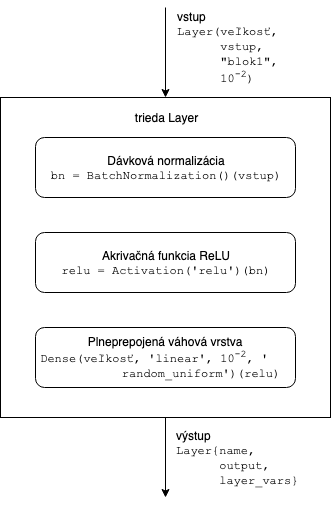
\includegraphics[width=0.4\textwidth]{images/skryta_vrstva.png}}
%popis obrazku
\caption[Implementačna architektúra skrytej vrstvy]{Implementačna architektúra skrytej vrstvy, ktorá pozostáva z niekoľkých podvrstiev. V našom prípade sa jedná o podvrstvu dávkovej normalizácie, podvrstvu s aktivačnou funkciou ReLU a plne-prepojenú váhovú vrstvu.}
\label{impl_vrstva}
%id obrazku, pomocou ktoreho sa budeme na obrazok odvolavat
\end{figure}

Objekt triedy \mintinline{Python}{Layer} ktorý je volaný za účelom vytvorenia skytej vrstvy, obsahuje tri atribútu:
\begin{enumerate}
    \item \mintinline{Python}{name} - názov vrstvy
    \item \mintinline{Python}{output} - váhová vrstva (výstup danej skrytej vrstvy)
    \item \mintinline{Python}{layer_vars} - váhy jednotlivých komponentov skrytej vsrtvy (vrstvy dávkovej normalizácie, vrstvy aktivačnej funkcie a váhovej vrstvy)
\end{enumerate}

Každá vytvorená vrstva je uložená do samostatnej premennej. Po vytvorení páru vrstiev (reziduálneho bloku) je vykonané sčítanie výstupu reziduálneho bloku (výstup párnej vrstvy z dvojice vrstiev) s identickým zobrazením. Identické zobrazenie predstavuje výsledok predchádzajúceho sčítania výstupu reziduálneho bloku s identickým prepojením, resp. vstupu MMD-ResNet ak sa jedná o prvý reziduálny blok v poradí (viď blok kódu na Obr. \ref{kod_vrstvy}). 

\begin{figure}
%vlozenie samotneho obrazku vycentrovaneho a vhodnej velkosti
%obrazok je v subore images/cervik.png
\centerline{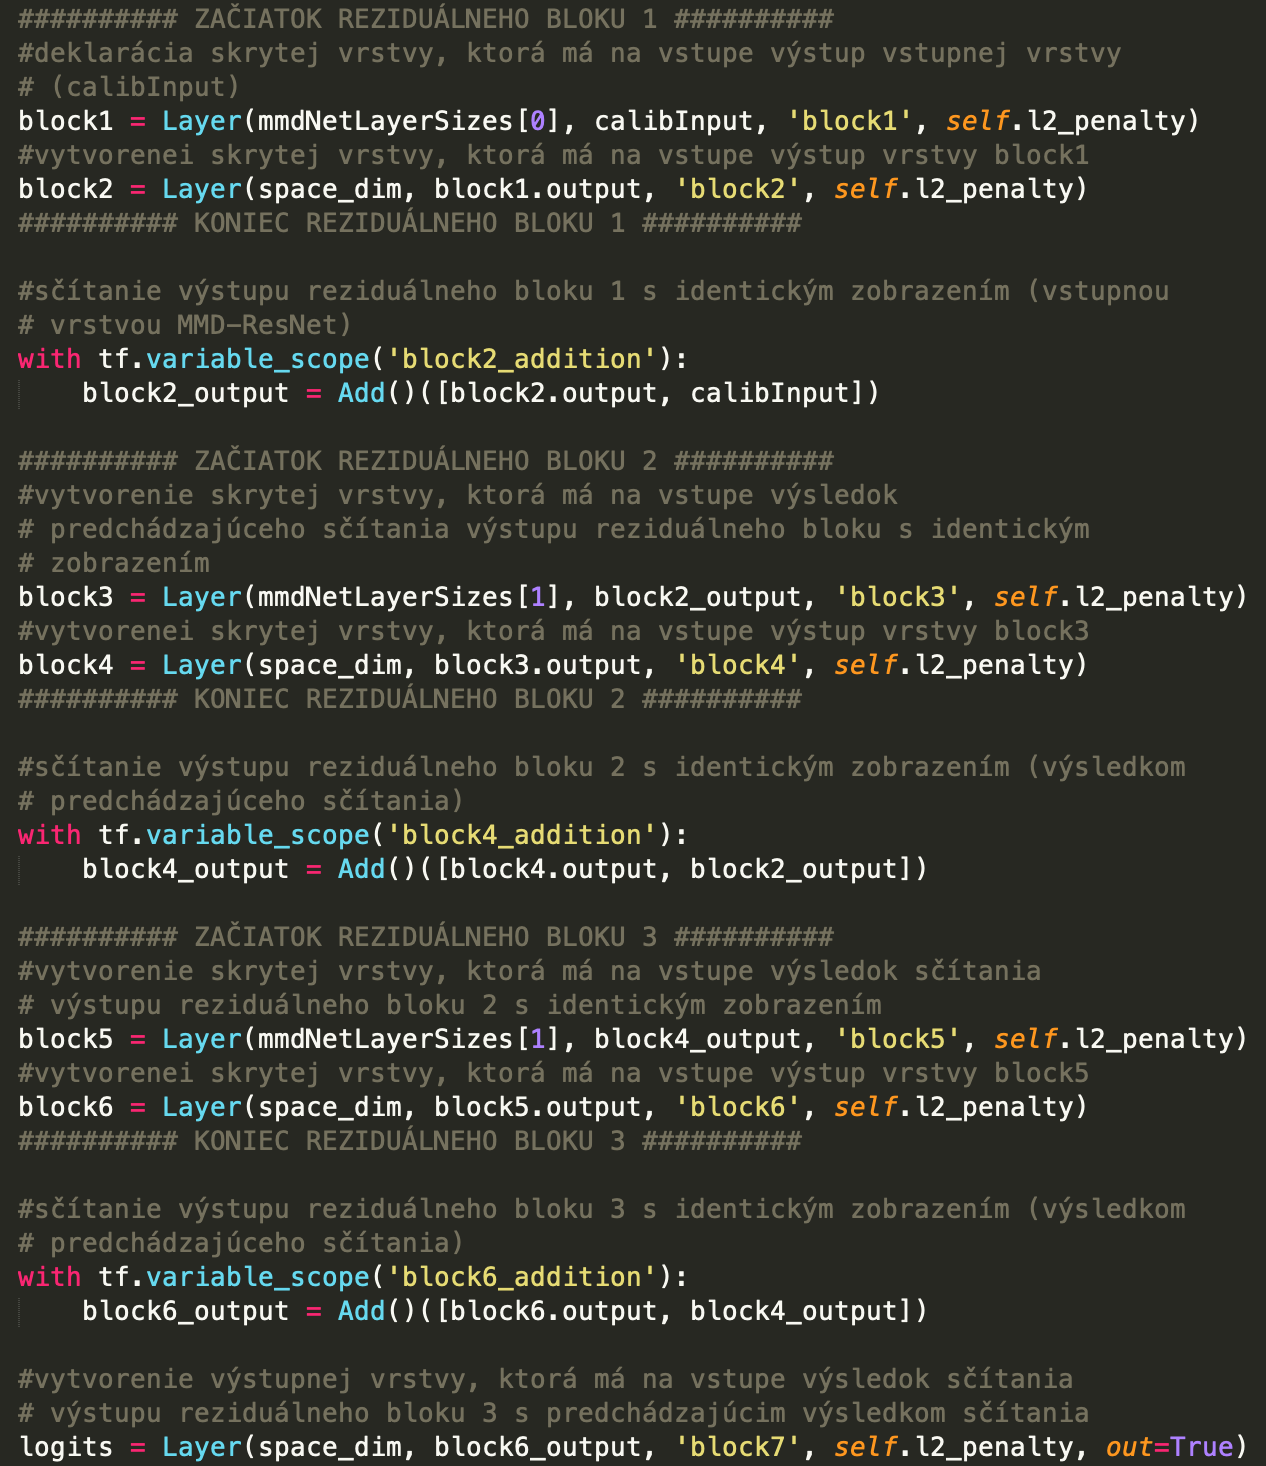
\includegraphics[width=0.8\textwidth]{images/kod.png}}
%popis obrazku
\caption[Deklarácia skrytých vrstiev MMD-ResNet]{Deklarácia jednotlivých skrytých vrstiev MMD-ResNet}
\label{kod_vrstvy}
%id obrazku, pomocou ktoreho sa budeme na obrazok odvolavat
\end{figure}

Sčítavanie výstupu reziduálneho bloku s identickým zobrazením je realizované funkciou \mintinline{Python}{Add()}, obsiahnutou v knižnici \mintinline{Python}{Keras}. Funkcia \mintinline{Python}{Add()} pijíma ako parameter pole vrstiev, ktorých výstup bude sčítaný.

Po deklarovaní všetkých vrstiev MMD-ResNet sú vrstvy priradené atribútu \mintinline{Python}{layers} triedy \mintinline{Python}{ModelSG()}.

Nasledujúcim krokom je vytvorenie modulov syntetického gradientu. Moduly syntetického gradientu sú realizované volaním konštruktora triedy \mintinline{Python}{Layer} (podobne ako v prípade štandardných skrytých vrstiev). Pri volaní konštruktora triedy \mintinline{Python}{Layer} v prípade tvorby modulov syntetického gradientu sú parametrami - veľkosť skrytej vrstvy, ktorej prislúcha daný modul syntetického gradientu, výstup skrytej vrstvy, ktorej prislúcha daný modul syntetického gradientu, názov modulu syntetického gradientu a identifikátor definujúci, že sa jedná o modul syntetického gradientu a nie o štandardnú skrytú vrstvu. Konštruktor triedy \mintinline{Python}{Layer} následne priradí danej vrstva špecifikovaný názov a vytvorí jednu plneprepojenú váhovú vrstvu (funkciou \mintinline{Python}{Dense()}, obsiahnutou v knižnici \mintinline{Python}{Keras}) s veľkosťou rovnou veľkosti priradenej skrytej vrstvy. Vstupom danej váhovej vrstvy je výstup skrytej vrstvy, ktorý je poskytnutý ako parameter pri volaní konštruktora. Objekt triedy \mintinline{Python}{Layer} má v každom prípade dostupné rovnaké atribúty (\mintinline{Python}{name}, \mintinline{Python}{output}, \mintinline{Python}{layer_vars}), rozdiel je len v architektúre vrstvy uloženej v atribúte \mintinline{Python}{output}. Zatiaľ čo štandardná skrytá vrstva obsahuje podvrstvu dávkovej normalizácie, podvrstvu s aktivačnou funkciou ReLU a váhovou vrstvou, tak vrstva pre modul syntetického gradientu obsahuje len jednu váhovú vrstvu.

Deklarované moduly syntetického gradientu sú priradené atribútu \mintinline{Python}{synth_layers}, triedy \mintinline{Python}{ModulSG}.

\section{Trénovanie MMD-ResNet}
\label{implementacia_trenovania_MMD_ResNet}

Po zostrojení všetkých skrytých vrstiev a im prislúchajúcim modulom syntetického gradientu nastáva fáza trénovania. Trénovanie je realizované metódou \mintinline{Python}{train()}. Metóda \mintinline{Python}{train()} prijíma ako parametre počet iterácii učenia, veľkosť dávky pre jednu iteráciu učenia, pravdepodobnosť aktivácie fázy spätného šírenia chyby a počiatočný krok učenia použitý pri úprave váh jednotlivých vrstiev a modulov syntetického gradientu.

V úvode trénovania sú metódou \mintinline{Python}{prepare_training()} inicializované tzv. optimalizátory trénovania. Optimalizátory deklarujú aktivity (resp. matematické operácie a transformácie dát), ktoré budú v priebehu trénovania vykonávané za účelom minimalizovania chyby neurónovej siete. V našom prípade ide o optimalizátory, ktoré definujú sekvencie aktivít vykonávaných za účelom 
\begin{enumerate}
    \item úpravy váh skrytých vrstiev MMD-ResNet pomocou syntetického gradientu (resp. pomocou výstupných hodnôt modulov syntetického gradientu)
    \item úpravy váh modulov syntetického gradientu pomocou syntetického gradientu predikovaného modulom syntetického gradientu z vyššej vrstvy
\end{enumerate}
tak, aby bolo dosiahnuté minimalizovanie hodnoty MMD.

Metóda \mintinline{Python}{prepare_training()} prijíma ako parametre krok učenia použitý pri úprave váh a hodnoty markerov referenčnej vzorku. Každý zadeklarovaný optimalizátor prislúcha aktívnemu virtuálnemu pamäťovému prostrediu v ktorom si ukladá všetky súkromné dáta. Optimalizátory zadeklarované v jednom virtuálnom prostredí nemôžu byť vykonané v inom virtuálnom prostredí.

Vzhľadom na použitie dynamicky sa meniaceho kroku učenia podľa definovaného rozvrhu je v aktívnom virtuálnom prostredí potrebné alokovať vymedzený priestor pre daný krok učenia. Vymedzenie priestoru pre jednu premennú je realizované funkciou \mintinline{Python}{Variable}, obsiahnutou v knižnici \mintinline{Python}{TensorFlow}. Funkcia \mintinline{Python}{Variable} prijíma ako parametre hodnotu danej premennej (počiatočná hodnotu kroku učenia), dátový typ premennej (\mintinline{Python}{float}) a názov premennej (\mintinline{Python}{lr}). Vytvorená premenná je priradená atributu \mintinline{Python}{learning_rate} triedy \mintinline{Python}{ModulSG}

Po alokovaní priestoru pre hodnotu kroku učenia je možné zadeklarovať optimalizátor, ktorý bude vykonávať regularizáciu kroku učenia o predom definovanú hodnotu. V našom prípade ide o optimalizátor, ktorý priraďuje premennej aktívneho virtuálneho prostredia nami definovanú hodnotu. Priradenie hodnoty premennej virtuálneho prostredia je realizované funkciou \mintinline{Python}{assign()}, obsiahnutou v knižnici \mintinline{Python}{TensorFlow}. Funkcia \mintinline{Python}{assign()} prijíma ako parametre premennú prostredia, ktorej bude priradená vybraná hodnota (v našom prípade premenná prostredia uložená pod atribútom \mintinline{Python}{learning_rate} triedy \mintinline{Python}{ModuleSG}), hodnota, ktorá bude priradená danej premennej (v našom prípade $\frac{learning\_rate}{lr\_div}$, kde $learning\_rate$ je hodnota premennej prostredia, uloženej pod atribútom \mintinline{Python}{learning_rate} triedy \mintinline{Python}{ModuleSG} a $lr\_div$ je hodnota regularizácie kroku učenia uložená pod atribútom \mintinline{Python}{lr_div} triedy \mintinline{Python}{ModuleSG}) a názov optimalizátora (\mintinline{Python}{lr_decrease}). Vytvorený optimalizátor je následne uložený do atribútu \mintinline{Python}{reduce_lr} triedy \mintinline{Python}{ModelSG}

Po vytvorení optimalizátora pre regularizáciu kroku je vytvorený optimalizátor výpočtu hodnoty MMD. Výpočet hodnoty MMD je realizovaný metódou \mintinline{Python}{KerasCost()}, triedy \mintinline{Python}{MMD} obsiahnutej v súbore \mintinline{Python}{CostFunction.py}. Volanie konštruktora triedy \mintinline{Python}{MMD} prijíma ako parametre výstup MMD-ResNet a hodnoty markerov z referenčnej vzorky, ktoré sú použité ako očakávaná hodnoty (supervízia). Volanie metódy \mintinline{Python}{KerasCost} nad inicializovaným objektom triedy \mintinline{Python}{MMD} vyráta hodnotu MMD medzi výstupom MMD-ResNet a hodnotou markerov v referenčnej vzorke, ktorá bola poskytnutá pri volaní konštruktora triedy \mintinline{Python}{MMD}.

Vytvorený optimalizátor výpočtu hodnoty MMD je ďalej použitý pri optimalizácii jednotlivých vrstiev MMD-ResNet. Optimalizácia jednotlivých vrstiev a modulov syntetického gradientu  je realizovaná pomocou metódy \mintinline{Python}{train_layer_n()} triedy \mintinline{Python}{ModelSG}. Metóda \mintinline{Python}{train_layer_n()} prijíma ako parametre:
\begin{enumerate}
    \item pozíciu vrstvy v zozname skrytých vrstiev (atribút \mintinline{Python}{layers}), ktorej váhy budú upravované 
    \item pozíciu vrstvy v zozname skrytých vrstiev (atribút \mintinline{Python}{layers}), ktorej výstup bude použitý pri vypočítavaní gradientu pre vrstvu ktorá bude upravovaná
    \item pozíciu modulu syntetického gradientu v zozname modulov syntetického gradientu (atribút \mintinline{Python}{synth_layers}), ktorého váhy budú upravované
    \item pozíciu vrstvy v zozname skrytých vrstiev (atribút \mintinline{Python}{layers}), ktorej váhy sú použité pri výpočte gradientu
    \item pozíciu modulu syntetického gradientu v zozname modulov syntetického gradientu (atribút \mintinline{Python}{synth_layers}), ktorý bude použitý pri ako počiatočný gradient úpravy váh skrytej vrstvy, ktorá bude upravovaná
\end{enumerate}
Volaním funkcie \mintinline{Python}{train_layer_n()} je deklarovaná séria optimalizérov, ktoré sú vzájomne poprepájané a následne reťazovo vykonávané. Prvý optimalizér konštruuje symbolické deriváty pomocou funkcie \mintinline{Python}{gradients()}, obsiahnutej v knižnici \mintinline{Python}{TensorFlow}. Symbolické deriváty sú vypočítavané z výstupných dát vyššej vrstvy od vrstvy ktorá je upravovaná v závislosti od výstupných dáta upravovanej vrstvy. Pri vyratávani symbolických derivátov je poskytnutý vlastný počiatočný gradient ktorý je reprezentovaný výstupom modulu syntetického gradientu generujúceho syntetický gradient pre vrstvu, ktorá bude upravovaná. Po vytvorení symbolických derivátov je deklarovaný optimalizátor hodnôt váh vrstvy, ktorá bude upravovaná. Optimalizátor hodnôt váh vrstiev je realizovaný funkciou \mintinline{Python}{RMSPropOptimalizer()}, obsiahnutý v knižnici \mintinline{Python}{TensorFlow}, ktorý berie ako parameter hodnotu kroku učenia. Symbolické derivácie ktoré boli vypočítané v predchádzajúcom kroku sú nasledne aplikované na optimalizátor hodnôt váh skrytých vrstiev funkciou \mintinline{Python}{apply_gradients()}, obsiahnutou v knižnici \mintinline{Python}{TensorFlow}. Funkcia \mintinline{Python}{apply_gradients()} prijíma ako parameter symbolické deriváty ktoré sú použité ako gradient na úpravu váh danej vrstvy. 

Po úprave váh skrytej vrstvy sú upravované váhy modulu syntetického gradientu. Modul syntetického gradientu vychádza zo symbolických derivátov vypočítaných pri úprave váh skrytej vrstvy, ktoré považuje za skutočný gradient. Prvotne je vytvorený optimalizátor, ktorý vypočítavá hodnotu chyby medzi skutočným gradientom (vypočítaným pri úprave váh skrytej vrstvy) a výstupom upravovaného modulu syntetického gradientu. Optimalizátor výpočtu hodnoty chyby predikcie modulu syntetického gradientu je realizovaný funkiou \mintinline{Python}{mean_squared_error()}, obsiahnutou v knižnici \mintinline{Python}{TensorFlow}. Funkcia \mintinline{Python}{mean_squared_error()} prijíma ako parametre predikované hodnoty (výstup modulu syntetického gradientu) a skutočné hodnoty (gradient vypočítaný pri úprave váh skrytej vrstvy).

Hodnota chyby je následne použitá pri deklarácii optimalizátora hodnôt váh modulu syntetického gradientu. Optimalizátor hodnôt váh modulu syntetického gradientu je realizovaný funkciou \mintinline{Python}{AdamOptimizer()}, obsiahnutou v knižnici \mintinline{Python}{TensorFlow}, ktorej vstupným parametrom je hodnota kroku učenia. Na daný optimalizátor je aplikovaná metóda \mintinline{Python}{minimize()}, obsiahnutá v knižnici \mintinline{Python}{Tensorflow}. Funkcia \mintinline{Python}{minimize()} prijíma ako parametre optimalizér ktorý vyrátava hodnotu chyby medzi predikovaným syntetickým gradientom (výstupom upravovaného modulu syntetického gradientu) a skutočným gradientom (vypočítaným pri úprave váh skrytej vrstvy) a váhy daného modulu syntetického gradientu, ktoré budú upravované za účelom znižovania hodnoty chyby predikcie.

Výstupom funkcie \mintinline{Python}{train_layer_n()} je dvojica optimalizátorov upravujúcich váhy skytej vrstvy a váhy modulu syntetického gradientu. Funkcia \mintinline{Python}{train_layer_n()} je volaná pre jednotlivé skryté vrstvy a im prislúchajúce moduly syntetického gradientu. Jednotlivé optimalizátory, ktoré boli deklarované funkciou \mintinline{Python}{train_layer_n()} sú uložené v pároch do atribútu \mintinline{Python}{decoupled_training}, triedy \mintinline{Python}{ModulSG}. 

Akonáhle sú deklarované všetky optimalizátory potrebné na trénovanie jednotlivých skrytých vrstiev MMD-ResNet, tak je možné vykonať ich inicializáciu. Inicializácia optimalizátorov je realizovaná funkciou \mintinline{Python}{global_variables_initializer()}, obsiahnutou v knižnici \mintinline{Python}{TensorFlow}.

Po inicializácii optimalizátorov je možné vykonávať jednotlivé akcie, ktoré dané optimalizátory deklarujú. Trénovanie MMD-ResNet využíva princíp spúšťania daných optimalizátorov vo vopred definovanom virtuálnom prostredí. Trénovanie prebieha iteratívnou formou, kde v každej iterácii je vykonané:
\begin{enumerate}
    \item Overenie podmienky vykonania zníženie hodnoty kroku učenia. Zníženie hodnoty kroku učenia je realizovené aktiváciou funkcie \mintinline{Python}{run()} nad aktívnym virtuálnym prostredím. Funkcia \mintinline{Python}{run()} prijíma ako parameter omptimalizér ktorý sa má vykonať. V našom prípade je to optimalizér uložený pod atribútom \mintinline{Python}{reduce_lr}, ktorý definuje akciu priradenia novej hodnoty kroku učenia do premennej prostredia uloženej pod atribúrom \mintinline{Python}{learning_rate} triedy \mintinline{Python}{ModelSG}
    \item Vytvorenie dávky dát použitej na trénovanie MMD-ResNet s veľkosťou definovanou pri volaní funkcie \mintinline{Python}{train()}.
    \item Samotné trénovanie jednotlivých skrytých vrstiev a modulov syntetického gradientu. Trénovanie spočíva v iterovaní dvojíc optimalizátorov uložených pod atribútom \mintinline{Python}{decoupled_training} triedy \mintinline{Python}{ModelSG}. Počas iterovania daných dvojíc je rovnako ako v prípade znižovania kroku učenia, použitá funkcia \mintinline{Python}{run()} nad aktívnym virtuálnym prostredím. Daná funkcia v tomto prípade prijíma ako parametre dvojicu optimalizátorov, ktoré sa majú paralelne vykonať (optimalizátor úpravy váh skrytej vrstvy a optimalizátor úpravy váh modulu syntetického gradientu). Volanie funkcie vyžaduje naplnenie priestoru alokovaného pre vstupné dáta. Naplnenie daného priestoru je realizované priradením dávky vstupných dát do parametra \mintinline{Python}{feed_dict} pri volaní funkcie \mintinline{Python}{run()}.
\end{enumerate}

Spúšťanie vykonávania jednotlivých dvojíc optimalizátorov umožňuje paralelizáciu trénovania jednotlivých vrstiev MMD-ResNet. V jednom čase sú vykonávané viaceré optimalizátory súčasne, pričom každý optimalízátor sekvenčne trénujú dvojicu - skrytá vrstvua a modul syntetického gradientu. Pri spustení vykonávania optimalizátora sú rekurzívne vykonané všetky optimalizátory, ktoré participujú pri deklarácii spúšťaného optimalizátora (vnorené optimalizátory). Pre lepšie pochopenie vnárania a rekurzívneho spúšťania optimalizátorov, viď Obr. \ref{rekurzivne}.

\begin{figure}
%vlozenie samotneho obrazku vycentrovaneho a vhodnej velkosti
%obrazok je v subore images/cervik.png
\centerline{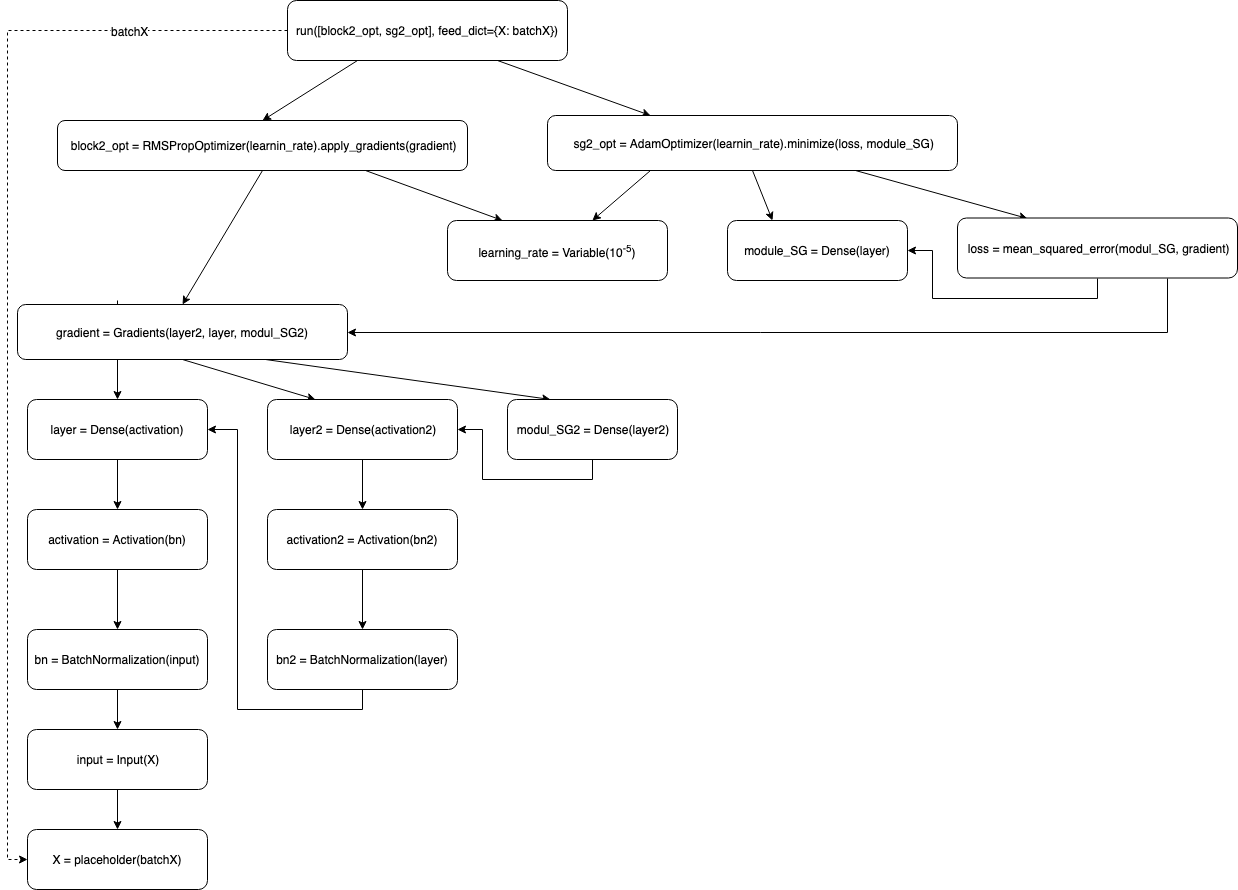
\includegraphics[width=1.0\textwidth]{images/rekurzivne.png}}
%popis obrazku
\caption[Ilustrácia rekurzívneho vykonávania vnorených optimalizátorov]{Ilustrácia rekurzívneho vykonávania vnorených optimalizátorov. Kód programu funkciou \mintinline{Python}{run()} spustil nad aktívnym virtuálnym prostredím vykonávanie optimalizátorov \mintinline{Python}{block2_opt} a \mintinline{Python}{sg2_opt}, pričom naplnil alokovaný priestor pre vstupné dáta hodnotou premennej \mintinline{Python}{batchX}. Vykonávané optimalizátory v tomto prípade predstavujú trénovanie 2. vrstvy modelu MMD-ResNet a modelu syntetického gradientu prislúchajúceho 1. vrstve. Obrázok ilustruje rekurzívne vykonávanie vnorených optimalizátorov, ktoré je nevyhnutné pre vykonanie akcie primárneho optimalizátora. Smer šípiek predstavuje smer volaní jednotlivých optimalizátorov. Z obrázka je možné vidieť, že optimalizátory, ktoré už boli vykonané v danom spustení primárneho optimalizátora, sú verejné a zdieľané medzi jednotlivými vnorenými optimalizátormi. Vnorené optimalizátory tak využívajú výsledky už vykonaných optimalizátorov a spustenia nového optimalizátora je realizované len v prípade, ak daný optimalizátor ešte nebol vykonaný.}
\label{rekurzivne}
%id obrazku, pomocou ktoreho sa budeme na obrazok odvolavat
\end{figure}

\section{Dátová sada}
\label{data_sets}

Model MMD-ResNet bol vo fáze implementácie trénovaný a testovaný na dátovej sade poskytnutej zdrojom \cite{Li2017}, dostupnej na adrese \url{https://github.com/KlugerLab/deepcytof/tree/master/Data/MultiCenter_16sample}. Dátova sada obsahuje kolekciu 16 vzoriek, ktoré sú uložené vo formáte \mintinline{Python}{CSV}. Jednotlivé vzorky sú rozdelené na dva súbory, pričom jeden súbor obsahuje hodnoty markerov jednotlivých buniek (súbory s prefixom \mintinline{Python}{sample}) a druhý súbor obsahuje identifikátory tried prislúchajúce daným bunkám (súbory s prefixom \mintinline{Python}{label}). Identifikátory tried tried boli získane manuálnym gatovaním každej vzorky \cite{Li2017}. 

Všetky vzorky boli merané na jednom testovacom subjekte v dvoch rôznych obdobiach a na rozličných meracích nástrojoch. V rámci trénovania a testovania MMD-ResNet sme vychádzali z markerov ktoré identifikoval zdroj \cite{Li2017} za relevantné. Celkovo sme použili 8 markerov: CCR6, CD20, CD45, CD14, CD16, CD8, CD3, CD4. Bunky opísané týmito markermi sme klasifikovali do 5 bunkových kategórií: B lymfocyty, CD4+ T lymfocyty, CD8+ T lymfocyty, monocyty a neurčité/neznáme bunky \cite{Li2017}.

Existujúcu implementáciu MMD-ResNet sme následne testovali na dátovej sade ktorú poskytla Slovenská Akadémia Vied. Dátová sada obsahovala 20 negatovaných vzoriek. Vzorky disponovali až 48 rôznymi markermi, z ktorých sme na základe odborného vedenia a konzultácií identifikovali 13 relevantných: CD34, CD10, CD19, CD27, IgM, IgD, CD138, CD20, CD22, IgG, IgA, CD38, CD45. Poskytnuté vzorky sa nám podarilo automaticky gatovať a čakáme na výsledky manuálneho gatovania vykonaného kompetentnými zamestnancami Slovenskej Akadémie Vied.

\section{Dodatočné úpravy a vylepšenia}

Pôvodná implementácia metódy DeepCyTOF ktorú poskytol zdroj \cite{Li2017} obsahovala zastaralé a nepodporované komponenty. Jedná sa predovšetkým o komponenty, ktoré sú obsiahnuté v knižniciach \mintinline{Python}{Scikit learn} a \mintinline{Python}{Keras}. Pre správne fungovanie metódy DeepCyTOF bolo nevyhnutné vyhľadať alternatívy za dané komponenty a upraviť implementáciu tak, aby bola zabezpečená kompatibilita s novými verziami jednotlivých knižníc.

\subsection{Úprava implementácie metódy DeepCyTOF}

Analýzou dátovej sady poskytnutej Slovenskou Akadémiou Vied sme identifikovali problém nekonzistencie štruktúry jednotlivých vzoriek v porovnaní so vzorkami dátovej sady ktorá bola prvotne používaná (viac v Kap \ref{data_sets}). Automatické gatovanie preto vyžadovalo úpravu spôsobu načítania jednotlivých vzoriek. Pri načítavaní sme znovupoužili funkciu \mintinline{Python}{loadDeepCyTOFData()}, obsiahnutú v súbore \mintinline{Python}{DataHandler.py}. Danú funkciu sme rozšírili o parameter definujúci počet riadkov ktoré majú byť ignorované pri načítavaní jednotlivých vzoriek. Funkcia pri načítaní vzorky dátovej sady ignoruje prvých $n$ riadkov, ktoré predstavujú názvy jednotlivých markerov obsiahnutých v danej vzorke, pričom $n$ je počet riadkov definovaný pri volaní funkcie \mintinline{Python}{loadDeepCyTOFData()}.

Pri prvotnom testovaní kalibrácie zdrojových vzoriek sme identifikovali problém pretrénovania klasifikátora, ktorý gatoval kalibrované zdrojové vzorky. Problém pretrénovaného klasifikátora spočíval v klasifikácii všetkých kalibrovaných buniek do majoritnej triedy. Problém sme sa prvotne rozhodli riešiť zníženim počtu iterácií trénovania klasifikátora a následne znížením hodnoty kroku učenia. Toto riešenie viedlo k nedotrénovaniu klasifikátora a následnému poklesu presnoti gatovania.

Daný problém sme následne riešili redukciou buniek majoritnej triedy. Redukciu vzoriek majoritnej triedy vykonáva funkcia \mintinline{Python}{uniformSamples()}, obsiahnutá v súbore \mintinline{Python}{DataHandler.py}. Funkcia \mintinline{Python}{uniformSamples()} prijíma ako parameter zvolenú vzorku dát. V našom prípade sme redukovali počet buniek majoritnej triedy referenčnú vzorky, ktorá je použitá na trénovanie bunkového klasifikátora. Redukciou buniek majoritnej triedy referenčnej vzorky sme dosiahli zvýšenie \textit{F1 skóre} pri klasifikácii kalibrovaných dát až o 30\%.

Pri implementácii MMD-ResNet využívajúcej algoritmus syntetického gradientu bolo potrebné nahradiť pôvodný model MMD-ResNet za nami vytvorený model. Pri tomto probléme sme pozmenili spôsob vykonávania vykonávania kalibrácie jednotlivých zdrojových vzoriek. Pôvodná implementácia MMD-ResNet bola realizovaná funkcionáne-orientovanou paradigmou, ktorú sme zamenili za objektovo-orientovanú paradigmu. Kalibrácia dát je realizovaná inicializáciou objektu triedy \mintinline{Python}{ModelSG}, obsiahnutej v súbore \mintinline{Python}{MMDNet_SG.py}, ktorá vykoná zostrojenie štruktúry MMD-ResNet, jej trénovanie a následne aj finálnu kalibráciu zdrojovej vzorky. Kalibrované dáta sú následne dostupné volaním atribútu \mintinline{Python}{output} triedy \mintinline{Python}{ModelSG}.

Pôvodný algoritmus DeepCyTOF neimplementoval funkcionalitu generovania výsledku automatické gatovania do súboru. My sme identifikovali tento problém ako kritický, keďže pôvodná implementácia neumožňuje archivovať výsledky automatického gatovania. Daný problém sme riešili implementáciou funkcie \mintinline{Python}{generateOutput()}, obisahnutej v súbore \mintinline{Python}{DataHandler.py}. Funkcia \mintinline{Python}{generateOutput()} prijíma ako parameter inicializovaný objekt triedy \mintinline{Python}{ModelSG}, výsledok gatovania kalibrovanej vzorky pomocou daného modelu a identifikátor zdrojovej vzorky. Výstupom funkcie sú:
\begin{itemize}
    \item zdrojové vzorky kalibrovaná pomocou MMD-ResNet s využitím algoritmu syntetického gradientu
    \item výsledok automatického gatovania (predikované triedy jednotlivých buniek zdrojovej vzorky)
    \item vyobrazenie vývoja hodnoty MMD a \textit{F1 skóre} v priebehu trénovania MMD-ResNet
\end{itemize}
Výstup funkcie \mintinline{Python}{generateOutput()} je zapísaný do súborov nachádzajúcich sa v adresári \mintinline{Python}{results}.

\subsection{Úprava implementácie syntetického gradientu v MMD-ResNet}
\label{uprava_implementacie_ResNet}

Zdroj \cite{Jaderberg2016} uviedol experiment v ktorom poskytol modulu syntetického gradientu dodatočnú informáciu v podobe supervízie prislúchajúcej aktuálne spracúvanej dávke (opísaný v Prílohe \ref{SGexperimets}). Naša implementácia zahŕňa poskytnutie dodatočnej implementácie modulu syntetického gradientu v podobe dát vybraných z referenčnej vzorky. Vzhľadom k tomu, že MMD-ResNet je trénovaná tak, aby minimalizovala rozdiel distribúcií hodnôt jednotlivých markerov medzi zdrojovou vzorkou a referenčnou vzorkou, tak referenčná vzorka sa v tomto prípade javí ako vhodná alternatíva za supervíziu.

Výber vhodných buniek použitých ako dodatočná informácia pre modul syntetického gradientu je realizovaný metódou \mintinline{Python}{getTargetsByClass()} triedy \mintinline{Python}{ModelSG}. Metóda \mintinline{Python}{getTargetsByClass()} prijíma ako parametre triedy buniek obsiahnutých v dávke určenej na trénovanie MMD-ResNet v danej iterácii (ďalej ako trénovacia dávka) a veľkosť trénovacej dávky. Funkcia \mintinline{Python}{getTargetsByClass()} vytvorí novú dávku s rovnakou dimenzionalitou ako trénovacia dávka. Vytvorená dávka obsahuje náhodne vybrané bunky z referenčnej vzorky, ktoré sú uložené do novovytvorenej dávky tak, aby ich triedy boli zhodné s triedami buniek trénovacej dávky na daných pozíciach. Napríklad, ak v trénovacej dávke je na pozícii 1 bunka z triedy \textit{monocyty}, tak v novovytvorenej dávke je na pozícii 1 náhodne vybraná bunka z referenčnej vzorky ktorá tiež patrí do triedy \textit{monocyty}. Výstupom funkcie \mintinline{Python}{getTargetsByClass()} je novovytvorená dávka.

Novovytvorená dávka (ďalej ako referenčná dávka) je použitá na naplnenie alokovaného priestoru deklarovaného pri konštruovaní MMD-ResNet. Referenčná dávka je v procese trénovania spájaná so vstupom jednotlivých modulov syntetického gradientu pomocou funkcie \mintinline{Python}{concatenate()}, obsiahnutej v knižnici \mintinline{Python}{Keras}. Spájanie referenčnej dávky so vstupom modulu syntetického gradientu je deklarované pri inicializácii modulu syntetického gradientu (pri volaní konštruktora triedy \mintinline{Python}{Layer}). 

Vzhľadom k tomu, že v rôznych iteráciach trénovania MMD-ResNet je v trénovacej dávke rôzne zastúpenie buniek z jednotlivých tried, tak funkcia \mintinline{Python}{getTargetsByClass()} je volaná v každej iterácii trénovania MMD-ResNet. Táto implementácia má negatívny vplyv na dĺžku trvania trénovania MMD-ResNet ale pozitívny vplyv na znižovanie hodnoty MMD (chybovej funkcie).

Vo fáze trénovania MMD-Resnet je po každých 10 iteráciach volaná funkcia \mintinline{Python}{checkState()}. Funkcia \mintinline{Python}{checkState()} vypočítavá hodnotu \textit{F1 skóre} v danej iterácii trénovania MMD-ResNet. Vypočítanie hodnoty \textit{F1 skóre} vychádza z validačných dát, ktoré sú kalibrované modelom MMD-ResNet v aktuálnej iterácii trénovania a následne gatované bunkovým klasifikátorok. Model MMD-ResNet si počas trénovania ukladá tú kópiu seba samého, ktorá pri klasifikácii kalibrovaných dát mala najvyššie \textit{F1 skóre}.

Aby sme dokázali lepšie využiť potenciál paralelného trénovania jednotlivých skrytých vrstiev MMD-ResNet, tak bolo potrebné trénovať MMD-ResNet na grafických akcelerátoroch. Trénovanie MMD-ResNet na procesore počítača nedovoľuje paralelné spúšťanie jednotlivých optimalizérov kvôli obmedzeniam vynútených operačným systémov. Spúšťanie optimalizérov je v našej implementácii riadené mechanizmami obsiahnutými v knižnici \mintinline{Python}{TensorFlow}. Nainštalovaním a importovaním knižnice \mintinline{Python}{MXNet} je umožnené mechanizmom knižnice \mintinline{Python}{TensorFlow} spúšťať optimalizátory na grafických akcelerátoroch. Knižnica \mintinline{Python}{MXNet} obsahuje sadu nástrojov ktoré sprístupňujú systémové prostriedky a tak umožňujú iným knižniciam prístup k výpočtovému jadru grafických akcelerátorov. Optimalizátory sú tak „odosielané“ na grafickú kartu, kde sú následne vykonávané. Vyspelé grafické akcelerátory obsahujú sadu inštrukcií prispôsobených na vykonávanie matematických operácií s maticami. Vykonávanie optimalizátorov na grafických akcelerátoroch je preto rýchlejšie.

Sprístupnenie grafického akcelerátora vyžaduje nainštalovanie ovládača NVIDIA\textsuperscript{\textregistered} GPU. Daný ovládač je možné nainštalovať len v prípade dostupnosti grafického čipu NVIDIA\textsuperscript{\textregistered}. Vzhľadom k tomu, že naše hardvérové možnosti nespĺňali tieto požiadavky, rozhodli sme sa využiť webovú službu Google Colaboratory. Služba Google Colaboratory umožňuje bezplatný prístup k výpočtovému výkonu grafických akcelerátorov NVIDIA\textsuperscript{\textregistered} Tesla. V prostredí Google Colaboratory sme následne vykonávali jednotlivé testovania.